\documentclass[./00PhotoBox.tex]{subfiles}
\graphicspath{{\subfix{./img/}}}
\begin{document}


\chapter{Voruntersuchungen}
\label{c:voruntersuchungen}
Vor und während des Aufbaues des eigentlichen Messystemes wurden einige Voruntersuchungen durchgeführt. Diese dienten dazu, die Machbarkeit des Systemes zu prüfen und die notwendigen Schritte zu ermitteln und zu optimieren. Hauptsächlich ging es hierbei um die Ermittlung der Kamerakonstanten und der Verzeichnung der Kamera. Auch wurde die Möglichkeit der Erstellung eines 3D-Modells durch Fokusstacking wurde untersucht. Die einzelnen Untersuchungen werden im Folgenden kurz vorgestellt.

\section{Änderung der Kamerakonstante durch Fokussierung}

\paragraph{These}
Die Kamerakonstante einer Kamera ändert sich durch die Fokussierung. Bei gleich eingestellter Objektdistanz ist die Kamerakonstante näherungsweise gleich sein.

\paragraph{Ziel}
In \citet[S. 59]{kraus} wird eine Formel (siehe \autoref{eq:kraus_fokus}) für die \Gls{Bildweite} b in Abhängigkeit des Gegenstandsweite g gegeben. Die Bildweite entspricht näherungsweise der Kamerakonstante \citep[S. 59]{kraus}. Die Nutzung der Formel als Näherungswert soll überprüft werden und eine optimierte Formel für die Raspberry Pi Kamera ermittelt werden.

\begin{align}
    \frac{1}{f} = \frac{1}{g} + \frac{1}{b}
    \label{eq:kraus_fokus}
\end{align}

\paragraph{Vorgehen}
Die Änderungen wurden in einem Versuch beobachtet. Hierzu wurde der Raspberry Pi Zero mit montierter Kamera fest vor einem Charuco-Kalibriermuster platziert. Dieser ermöglicht auch bei unscharfen Bildern noch eine gute automatische Erkennung der zu beobachtenden Punkte. Es wurden je 11 Bilder mit unterschiedlichen Fokussierungen von $2~\text{m}$ bis  $10~\text{cm}$ aufgenommen. Dieser Vorgang wurde insgesamt viermal wiederholt, um auch die Wiederholungsgenauigkeit zu ermitteln. Die Bilder wurden anschließend mit einem Python-Script unter Nutzung von OpenCV ausgewertet. Hierbei wurde die relative Veränderung der Kamerakonstante der Kamera ermittelt und mit dem erwarteten Wert verglichen. Die relativen Änderungen wurden auf eine Fokusdistanz von $20~\text{cm}$ (entspricht einer Kamerakonstante von $5~\text{dpt}$) normiert. Relative Angaben wurden genutzt, da noch keine Kamerakonstante zu dem Zeitpunkt vorlag oder angenommen werden sollte.

\paragraph{Ergebnis}
Die Ergebnisse sind in \autoref{img:fokus_faktor} dargestellt. Es zeigt sich, dass die Änderungen der Kamerakonstante durch die Fokusierung linear zu der Dioptrienzahl (Kehrwert der Gegenstandsweite) sind. Ein lineares Verhältnis ergibt sich auch mit der im Datenblatt angegebenen Brennweite von $4,74~\text{mm}$, jedoch eine etwas flachere Gerade (blau). Die ausgleichende Gerade (blau) ergab eine Brennweite von $6,97~\text{mm}$. Die Abweichung von $2,23~\text{mm}$ entspricht einer Abweichung von $47\%$, was als unrealistisch hoch eingeschätzt wird. Hier scheinen sich weitere Effekte bemerkbar zu machen, die noch nicht berücksichtigt wurden. Es wurde daher auch die Verzeichnung weiter untersucht.

\begin{figure}
    \centering
    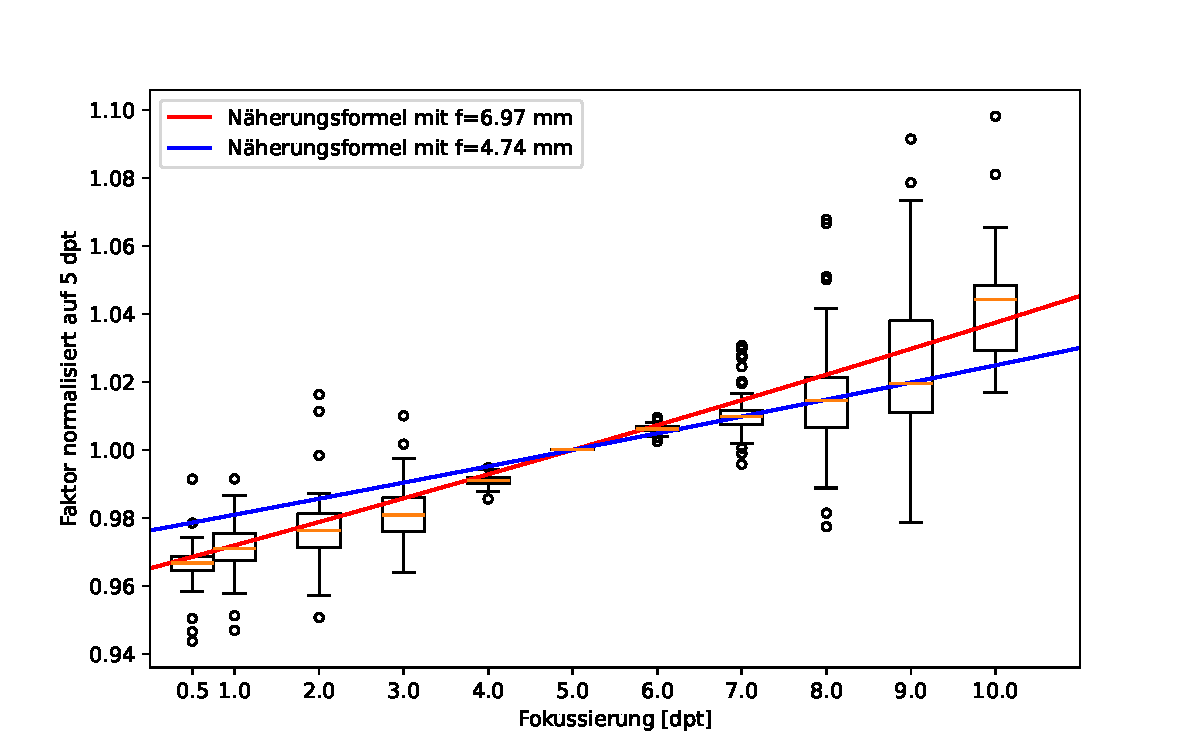
\includegraphics[width=1\textwidth]{./img/fokus_faktor_diagramm_box.pdf}
    \caption{Box-Whisker-Plot der relativen Veränderung der Kamerakonstante normalisiert auf eine Fokusdistanz von 20 cm (5 dpt)} %Bildunterschrift
    \label{img:fokus_faktor} %ID fürs Bild
\end{figure}



\section{Änderung der Verzeichnung mittels Charuco-Board}

\paragraph{These}
Durch die Verschiebung der Linsen beim Fokusieren verändert sich auch die Verzeichnung der Kamera.

\paragraph{Ziel}
Die Veränderung der Verzeichnung soll ermittelt und eine Korrekturformel ermittelt werden.

\paragraph{Vorgehen}
Der Versuchsaufbau von der Bestimmung der relativen Änderung der Kamerakonstante blieb bestehen. Es wurden jedoch zusätzlich die Verzeichnungen der Bilder ermittelt. Die Verzeichnung wurde mit OpenCV ermittelt und mit der erwarteten Verzeichnung verglichen.

\paragraph{Ergebnis}
Die Ergebnisse waren nicht zufriedenstellend. Es zeigte sich, dass die Verzeichnung mit nur einer Aufnahme pro Fokussierung nicht zufriedenstellend modelliert werden konnte.

\section{Bestimmung des Zusammenhang zwischen innerer Orientierung und Fokussierung}

\paragraph{These}
Die innere Orientierung ist von der Fokussierung abhängig.

\paragraph{Ziel}
Es soll eine Formel zur Bestimmung von Näherungswerten für die innere Orientierung in Abhängigkeit der Fokussierung ermittelt werden.

\paragraph{Vorgehen}
Es wurden mit fünf verschiedenen Fokussierungen mit jeweils 24 Raspberry-Pi-Kameras Bilder aufgenommen und die Bilder in Agisoft Metashape mittels Aruco-Marker orientiert, dessen Position bekannt war (siehe \autoref{sec:kalibrierung}). Außerdem wurden etwa 100 Schneider-Marker im Bildbereich der Kameras verteilt und als Verknüpfungspunkte benutzt. Es wurde jeweils in Metashape alle Bilder mit der gleichen Fokussierung als eine Kamera angenommen und die innere Orientierung bestimmt. Anschließend wurden alle Kameras nochmal einzeln ausgeglichen. Die innere Orientierung wurde in Form von Brennweite, Bildhauptpunktverschiebung und Verzeichnung ermittelt. Die Ergebnisse wurden in einem Box-Whisker-Plot dargestellt und eine ausgleichende Gerade ermittelt.

\paragraph{Ergebnis}

Die Ergebnisse sind in \autoref{img:naeherungswerte} dargestellt. Wie auch schon in der vorherigen Untersuchung zeigt sich, dass die Brennweite linear zur Fokussierung ist. Bei der Bildhauptpunktverschiebung und der Verzeichnung ist die Abhängigkeit nicht eindeutig. \autoref{tab:naeherungswerte_corr} zeigt die Korrelationsmatrix der Näherungswerte. Es zeigt sich, dass die Fokussierung und die Brennweite stark korreliert sind. Die Bildhauptpunktverschiebung ist nur schwach korreliert. Die Verzeichnung ist nicht korreliert. Es zeigt sich, dass die innere Orientierung durch die Fokussierung beeinflusst wird. Die Brennweite ist dabei erwartungsgemäß am stärksten betroffen.

\begin{figure}
    \centering
    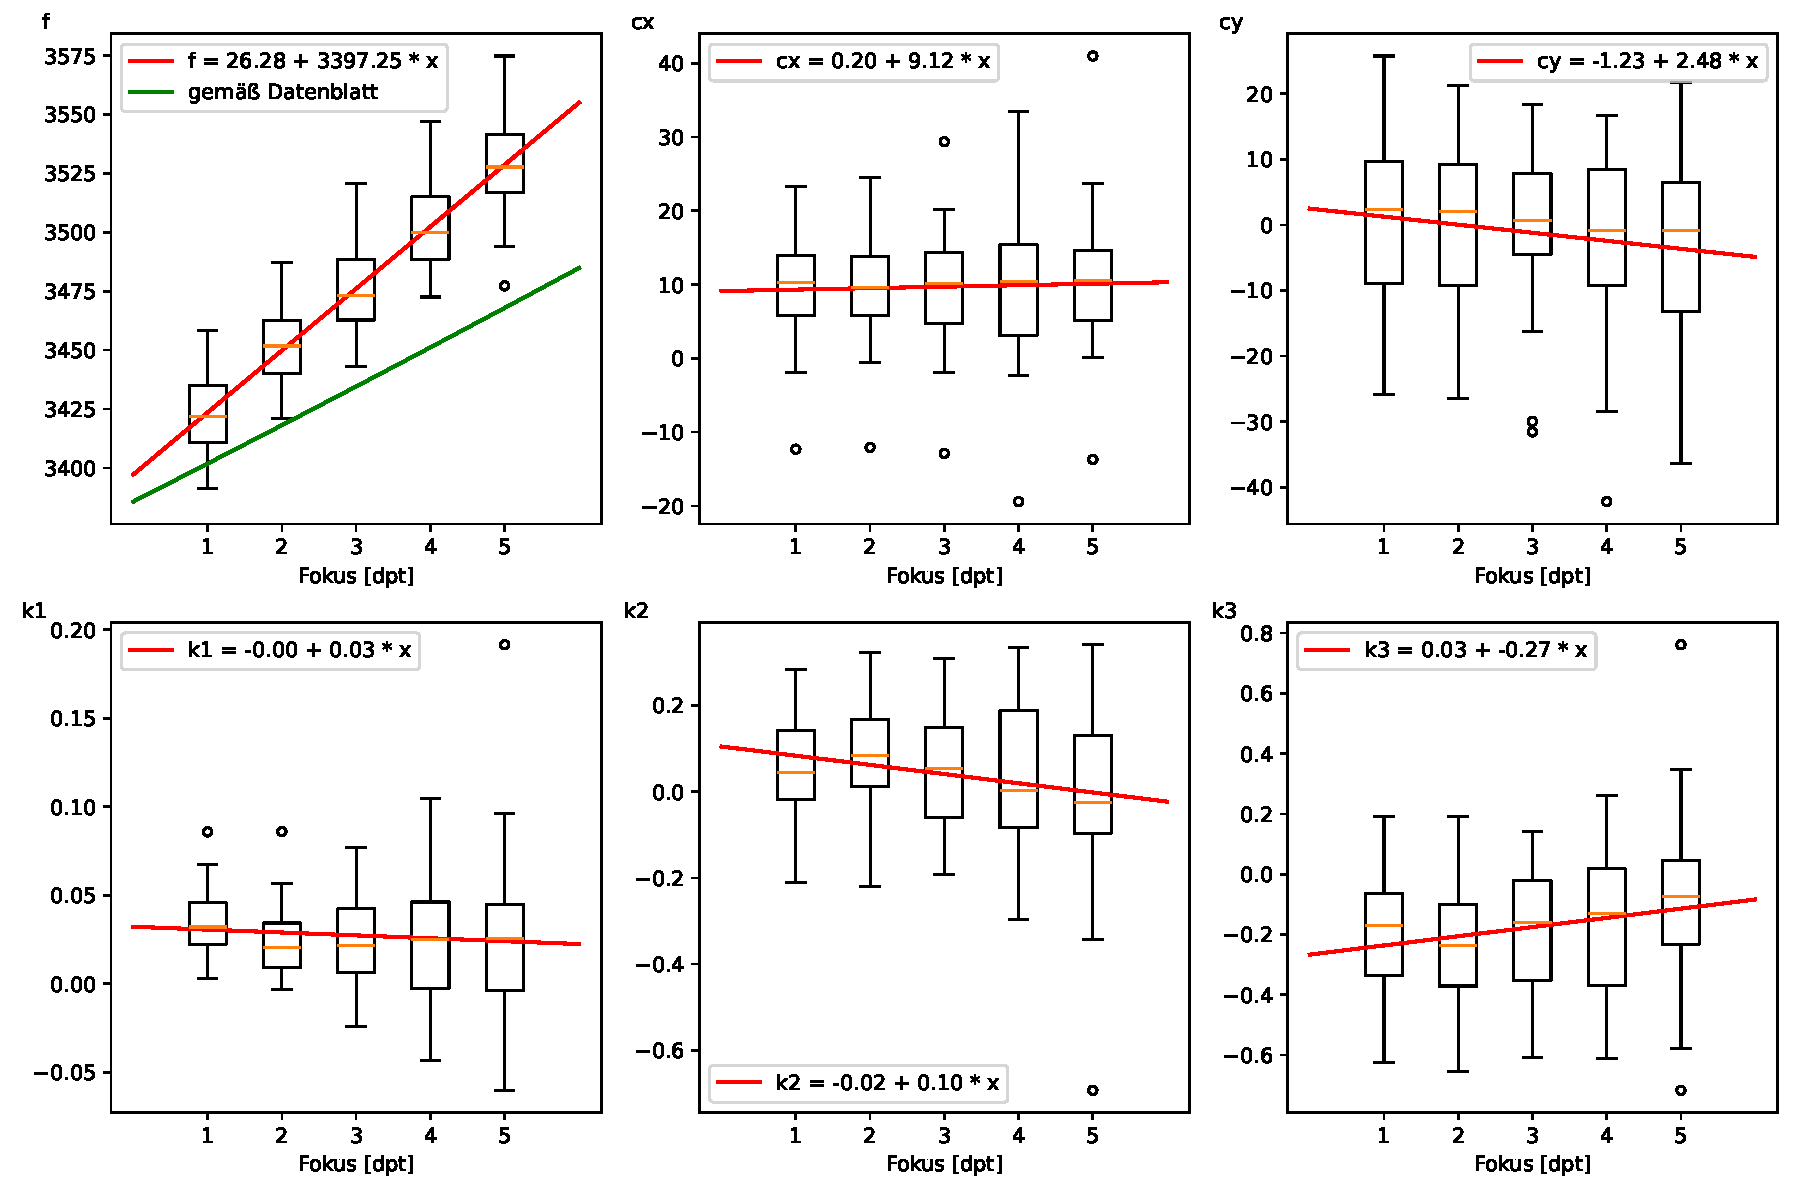
\includegraphics[width=1\textwidth]{./img/naeherungswerte_diagramm.pdf}
    \caption{Box-Whisker-Plots und ausgleichende Gerade der inneren Orientierung in Abhängigkeit von der Fokussierung [dpt]} %Bildunterschrift
    \label{img:naeherungswerte} %ID fürs Bild
\end{figure}

\begin{table}
\caption{Korrelationsmatrix der Näherungswerte}
\label{tab:naeherungswerte_corr}
\begin{tabular}{lrrrrrrr}
\toprule
 & Fokus [dpt] & f & cx & cy & k1 & k2 & k3 \\
\midrule
Fokus [dpt] & 1,000 & 0,901 & 0,032 & -0,128 & -0,069 & -0,181 & 0,177 \\
f &   & 1,000 & -0,010 & -0,211 & -0,220 & -0,071 & 0,092 \\
cx &   &   & 1,000 & -0,230 & 0,005 & 0,005 & 0,005 \\
cy &   &   &   & 1,000 & 0,031 & 0,023 & -0,051 \\
k1 &   &   &   &   & 1,000 & -0,925 & 0,866 \\
k2 &   &   &   &   &   & 1,000 & -0,985 \\
k3 &   &   &   &   &   &   & 1,000 \\
\bottomrule
\end{tabular}
\end{table}


\section{3D-Modell aus Fokusstacking}

\paragraph{These}
Durch Fokusstacking kann ein besseres 3D-Modell erstellt werden.

\paragraph{Ziel}
Es soll geprüft werden, ob durch Fokusstacking die Qualität des 3D-Modell verbessert werden kann. Hierzu wird ein 3D-Modell aus einem Fokusstacking erstellt und mit einem normalen 3D-Modell verglichen.

\paragraph{Vorgehen}
\begin{itemize}
    \item Automatisierter Fokusstacking
    \item keine Beachtung der festen Ausrichtung
    \item Transformation über SIRF und Homographie
\end{itemize}
\todo{Textform}

\paragraph{Ergebnis}
\todo{Füllen}

\biblio
\end{document}